\documentclass[a4paper]{article}
\usepackage{amsfonts}
\usepackage{amsmath}
\usepackage{amssymb}
\usepackage{graphicx}     

\begin{document}
  
\noindent \large Auteur: Stan Van Campenhout \\
\noindent \large Studierichting:  Informatica\\
\noindent \large Oefeningenreeks 5G nr. 16.2\\

\medskip

\normalsize

\begin{figure}[h]
\centering
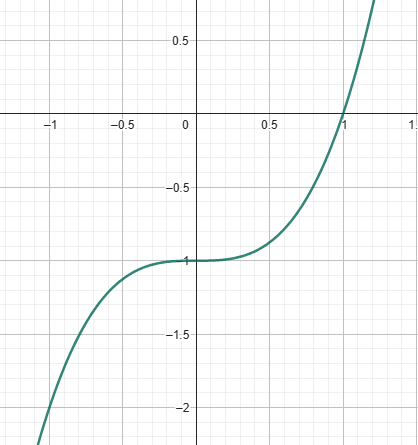
\includegraphics[width=5cm]{5G-16.2-stan.van.campenhout.INF.png}

\end{figure}

$ y = x^3 $ rond $ y = 1 \Rightarrow y = x^3 - 1 $ rond de x-as over $ \left[1,3\right] $\\

$ \Rightarrow \pi\displaystyle\int_1^3\left(x^3-1\right)^2dx = \pi\displaystyle\int_1^3\left(x^6-2x^3+1\right)dx = \pi\left[\dfrac{x^3}{7} - \dfrac{x^4}{2} + x\right]_1^3 $\\

$ = \pi\left(\dfrac{3849}{14} - \dfrac{9}{14}\right) = \dfrac{1920\pi}{7} $\\

\begin{thebibliography}{999}
%\bibitem{a} Referentie
\end{thebibliography}
\end{document} 
